\documentclass{beamer}

% Russian-specific packages
%--------------------------------------
\usepackage[T2A]{fontenc}
\usepackage[utf8]{inputenc}
\usepackage[russian]{babel}

\hypersetup{
    unicode=true % otherwise get "Glyph not defined"
}
%--------------------------------------

% Asymptote for pictures
%--------------------------------------
\usepackage{asymptote} %% comes with options inline and attach
%--------------------------------------


% graphicx for graphs
%--------------------------------------
\usepackage{graphicx}
\usepackage{subfig}
\graphicspath{
    {./pic/}
}
%--------------------------------------

\usetheme{default}

\newtheorem{stmt}{Утверждение}
\newtheorem{prblm}{Затруднение}
\definecolor{Periwinkle}{HTML}{4444AC}

\title{Движение симметричного экипажа \\с массивными роликами на омни-колесах}

\author{К.В. Герасимов, А.А. Зобова,  И.И.Косенко}

\institute[мех-мат МГУ]
{
  Кафедра теоретической механики и мехатроники\\
  Механико-математический факультет\\
  МГУ им. М.В. Ломоносова
}

\date{Ломоносовские чтения, 2017}

% Delete this, if you do not want the table of contents to pop up at
% the beginning of each subsection:
\AtBeginSubsection[]
{
  \begin{frame}<beamer>{План}
    \tableofcontents[currentsection,currentsubsection]
  \end{frame}
}

% Let's get started
\begin{document}

\begin{frame}
  \titlepage
\end{frame}

\begin{frame}{План}
  \tableofcontents
  % You might wish to add the option [pausesections]
\end{frame}


\section{Постановка задачи}

\begin{frame}{Постановка задачи}{Рисунки}
    \begin{figure}
        \centering
        \minipage{0.5\textwidth}
            \asyinclude{pic_cart.asy}
            \caption{Экипаж}
        \endminipage
        \minipage{0.5\textwidth}
            \asyinclude{pic_wheel.asy}
            \caption{Колесо}
        \endminipage
    \end{figure}
\end{frame}

\begin{frame}{Постановка задачи}{Тела, связи, степени свободы}
  \begin{itemize}
  \item {
    Экипаж состоит из платформы, $N$ колес и $n$ роликов,\\
    количество твердых тел:
    $$1 + N(n+1)$$
  }
  \item{
    Оси и центры колес и роликов неподвижны относительно\\
    платформы и колес соответственно
  }
  \item {
    Скорость точек контакта равна нулю:
    $$\vec{v}_{C_i} = 0, i = 1\dots N$$
  }
  \item{
    Количество степеней свободы:
    $$3 + N(n-1)$$
  }

  \end{itemize}
\end{frame}

\begin{frame}{Постановка задачи}{Координаты, псевдоскорости, связи}
  \begin{itemize}
  \item {
    Обобщенные координаты: \\
    $q = (x, y, \theta, \chi_i, \phi_k, \phi_s),$ где $i,k = 1\dots N$, $s$ -- ролики вне контакта.
  }
  \item{
    Псевдоскорости:\\
    $\nu = (\nu_1, \nu_2, \nu_3, \nu_s), \vec{v}_S = R\nu_1\vec{e}_\xi + R\nu_2\vec{e}_\eta, \nu_3 = \Lambda\dot{\theta}, \nu_s = \dot{\phi}_s$
  }
  \item {
    Связи:
	$$ \dot{x} = R \nu_1\cos\theta-R\nu_2\sin\theta, \hspace{15pt} \dot{y} = R\nu_1\sin\theta+R\nu_2\cos\theta,$$
	$$\dot{\theta} = \frac{\nu_3}{\Lambda}, \hspace{15pt} \dot{\chi}_i = \frac{R}{l}(\nu_1\sin\alpha_i - \nu_2\cos\alpha_i - \frac{\nu_3}{\Lambda}), $$
	$$ \dot{\phi_k} = \frac{R}{l\cos\chi_k-r}(\nu_1\cos\alpha_k + \nu_2\sin\alpha_k), \hspace{15pt} \dot{\phi}_s = \nu_s $$
  }

  \end{itemize}
\end{frame}

\section{Уравнения движения}

\subsection{Кинетическая энергия и лагранжиан}

\begin{frame}{Кинетическая энергия и лагранжиан}
  \begin{itemize}
  \item {
    Присутствует аддитивный член, пропорциональный $B$ -- моменту инерции ролика относительно его оси собственного вращения:
    $$ 2T = 2L = M\vec{v}_S^2 + I_S\dot{\theta}^2 + J\sum_i\dot{\chi}_i^2 + $$
    $$ + \alert{B\sum_{i,j}(\dot{\phi}_{ij}^2 + 2\dot{\theta}\sin(\kappa_j + \chi_i)\dot{\phi}_{ij})}, $$
    $$ M = \mathring{M} + Nnm $$
    $$ I_S = \mathring{I_S} + N\cdot n(\frac{A+B}{2} + mR^2 + \frac{mr^2}{2}), $$
    $$ J = \mathring{J} + n(A + mr^2) $$
  }

  \end{itemize}
\end{frame}

\begin{frame}{Кинетическая энергия и лагранжиан}
  \begin{itemize}
  \item {
    С учетом связей:
    $$ 2L^{*} = \mathring{\nu}^T \mathring{V}^T \mathring{M} \mathring{V} \mathring{\nu} + $$
    $$ + \alert{B}\sum_{i}(
    	\frac{(\nu_2\sin\alpha_i+\nu_1\cos\alpha_i)^2R^2}
    	{\rho_i^2} + $$
    $$ +
    	\frac{2R\nu_3(\nu_2\sin\alpha_i+\nu_1\cos\alpha_i)\sin\chi_i}
    	{\rho_i\Lambda}
    ) $$
    $$ +
    \alert{B}\sum_{i,j}(
    	\frac{2\nu_3\nu_{ni+j}\sin(\kappa_j+\chi_i)}
    	{\Lambda}
    	+
    	\nu_{ni+j}^2
    )
    $$
    где $ \frac{1}{2}\mathring{\nu}^T \mathring{V}^T \mathring{M} \mathring{V} \mathring{\nu} $ -- лагранжиан системы без роликов, $\rho_i = l\cos\chi_i - r$
  }

  \end{itemize}
\end{frame}

\begin{frame}{Кинетическая энергия и лагранжиан}{Матрицы кинетической энергии и связей для системы без роликов}
    $$ \mathring{M} = diag(M, M, I_S, J...J), $$
    $$ \mathring{V} = \begin{bmatrix}
        R\cos\theta & -R\sin\theta & 0 \\
        R\sin\theta & R\cos\theta  & 0 \\
        0           & 0            & \frac{1}{\Lambda} \\
        \frac{R}{l}\sin\alpha_i & -\frac{R}{l}\cos\alpha_i & -\frac{R}{l\Lambda} \\
    \end{bmatrix} $$
\end{frame}

\subsection{Структура уравнений - отличие от случая без роликов}

\begin{frame}{Структура уравнений}{Отличие от случая без роликов}
  \begin{itemize}
  \item {
    Уравнения Я.В. Татаринова:
    $$ \frac{d}{dt}\frac{\partial L^{*}}{\partial \nu_\alpha}  + \{P_\alpha, L^{*}\} = \{P_\alpha, \nu_\mu P_\mu\}, $$
    $$ \nu_\mu P_\mu = \dot{q_i} p_i, \hspace{10pt} p_i = \frac{\partial L}{\partial \dot{q}_i} $$
  }
  \item {
    Лагранжиан и ``импульсы'' отличаются аддитивными членами:
    $$ L^{*} = \mathring{L}^{*} + BL^{*}_\Delta(\nu, \chi) $$
    $$ P_\alpha = \mathring{P_\alpha}(\theta, p_x, p_y, p_\chi) + P_\Delta(p_{\phi_i}, \chi) $$
  }

  \end{itemize}
\end{frame}

\begin{frame}{Структура уравнений}{Отличие от случая без роликов}
     \begin{stmt}
    Учет массы роликов приводит к появлению в правой части дифференциальных уравнений, описывающих динамику экипажа, слагаемых, пропорциональных собственному моменту инерции роликов $B$ и квадратично зависящих от псевдоскоростей. Эти новые слагаемые явно зависят от углов поворота колес $\chi_i$.
    $$\boldsymbol{A}\dot{\boldsymbol{\nu}} = \frac1\Lambda
    \left(
    \begin{array}{c}
         \nu_2\nu_3  \\
         -\nu_1\nu_3 \\
         0
    \end{array}
    \right) + \alert{B}
     \left(
    \begin{array}{c}
         \boldsymbol{\nu}^T\boldsymbol{F}_1(\chi_i)\boldsymbol{\nu}  \\
         \boldsymbol{\nu}^T\boldsymbol{F}_2(\chi_i)\boldsymbol{\nu} \\
         \boldsymbol{\nu}^T\boldsymbol{F}_3(\chi_i)\boldsymbol{\nu}
    \end{array}
    \right)
    $$
    $$
    \dot{\chi}_i = \frac{R\sin\alpha_i}{l}\nu_1 - \frac{R\cos(\alpha_i)}{l}\nu_2 - \frac{R}{l\Lambda}\nu_3, \quad i = 1..N
    $$
    $$
    \Lambda\dot{\nu}_{ni+j} = -\dot{\nu}_3\sin(\chi_i+\kappa_j) - \dot{\chi_i}\nu_3\cos(\chi_i+\kappa_j), \quad j = 2..n
    $$
    \end{stmt}
\end{frame}

\begin{frame}{Структура уравнений}{Отличие от случая без роликов}    
    $$\boldsymbol{A}\dot{\boldsymbol{\nu}} = \frac1\Lambda
    \left(
    \begin{array}{c}
         \nu_2\nu_3  \\
         -\nu_1\nu_3 \\
         0
    \end{array}
    \right) + \alert{B}
     \left(
    \begin{array}{c}
         \boldsymbol{\nu}^T\boldsymbol{F}_1(\chi_i)\boldsymbol{\nu}  \\
         \boldsymbol{\nu}^T\boldsymbol{F}_2(\chi_i)\boldsymbol{\nu} \\
         \boldsymbol{\nu}^T\boldsymbol{F}_3(\chi_i)\boldsymbol{\nu}
    \end{array}
    \right)
    $$
    
    \textcolor{Periwinkle}{Доказательство:}
%   \begin{proof}
  $$ \frac{d}{dt}\frac{\partial L^{*}}{\partial \nu_\alpha} = - \{P_\alpha, L^{*}\} + \{P_\alpha, \nu_\mu P_\mu\},$$
    $$ \frac{d}{dt}\frac{\partial }{\partial \nu_\alpha}(L^{*} - \mathring{L^{*}}) = \alert{B}\frac{d}{dt}\frac{\partial}{\partial \nu_\alpha}L^{*}_\Delta(\nu, \chi), $$
    $$ \{P_\alpha, L^{*}\} - \{\mathring{P}_\alpha, \mathring{L}^{*}\} = \alert{B}\{ P_\alpha, L^{*}_\Delta(\nu, \chi) \} $$
    $$\rho_i = l\cos\chi_i - r, \quad \{P_\alpha, P_\mu\} - \{\mathring{P}_\alpha, \mathring{P}_\mu\}  = $$
    $$ = \alert{B}\frac{R^2}{\Lambda}\sum_i\frac{f_\alpha(\nu, \chi)}{\rho^2_i}(\frac{R}{\rho_i}(\nu_1\cos\alpha_i + \nu_2\sin\alpha_i) + \frac{\sin\chi_i}{\Lambda}\nu_3)$$
%  \end{proof}
\end{frame}

\section{Численное решение}

\subsection{Переход между роликами}

\begin{frame}{Переход между роликами}{Сложности и допущения}
    \textcolor{Periwinkle}{(1) Уравнения вырождаются на стыках роликов:}\\
    \textit{квадратичные формы $\boldsymbol{F}_i$ терпят разрыв 2ого рода из-за выражений $(l\cos\chi_i-r)$ в знаменателе.} \\
    Пусть переход на следующий ролик будет раньше стыка.
    \begin{figure}
        \centering
        \asyinclude{pic_overlap.asy}
        \caption{Ролики перекрываются}
    \end{figure}
\end{frame}

\begin{frame}{Переход между роликами}{Сложности и допущения}
    \textcolor{Periwinkle}{(2) Ролики входят и выходят из состояния контакта.}\\
    Будем рассматривать только движение роликов в контакте.\\
    Отбросим уравнения
    $$
    \Lambda\dot{\nu}_{ni+j} = -\dot{\nu}_3\sin(\chi_i+\kappa_j) - \dot{\chi_i}\nu_3\cos(\chi_i+\kappa_j), \quad j = 2..n.
    $$
    При переходе сохраним значения $\nu_1$, $\nu_2$, 
    $\nu_3$, а $\dot\chi_i$ пересчитаем по уравнениям связей.
    \begin{figure}
        \centering
        \asyinclude{pic_change.asy}
    \end{figure}
\end{frame}


\subsection{Примеры. Сравнение со случаем без роликов}

\begin{frame}{Вращение вокруг своей оси ($\nu_{1,2}(0) = 0, \nu_3 = 1$)}{Экипаж без роликов}
    \begin{columns}
        \column{0.33\textwidth}
            \centering
            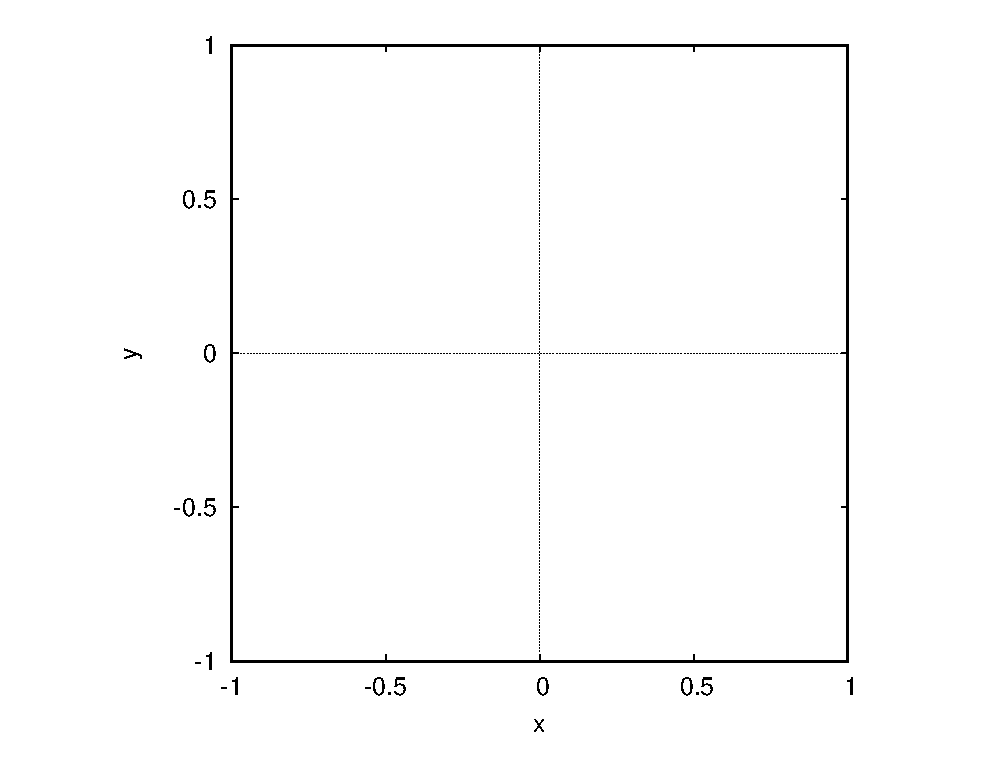
\includegraphics[width=\linewidth, height=30mm]{_old_sol__0_0_1__0__10__1e2_trajectory} \\
            Траектория $X, Y$ \\
            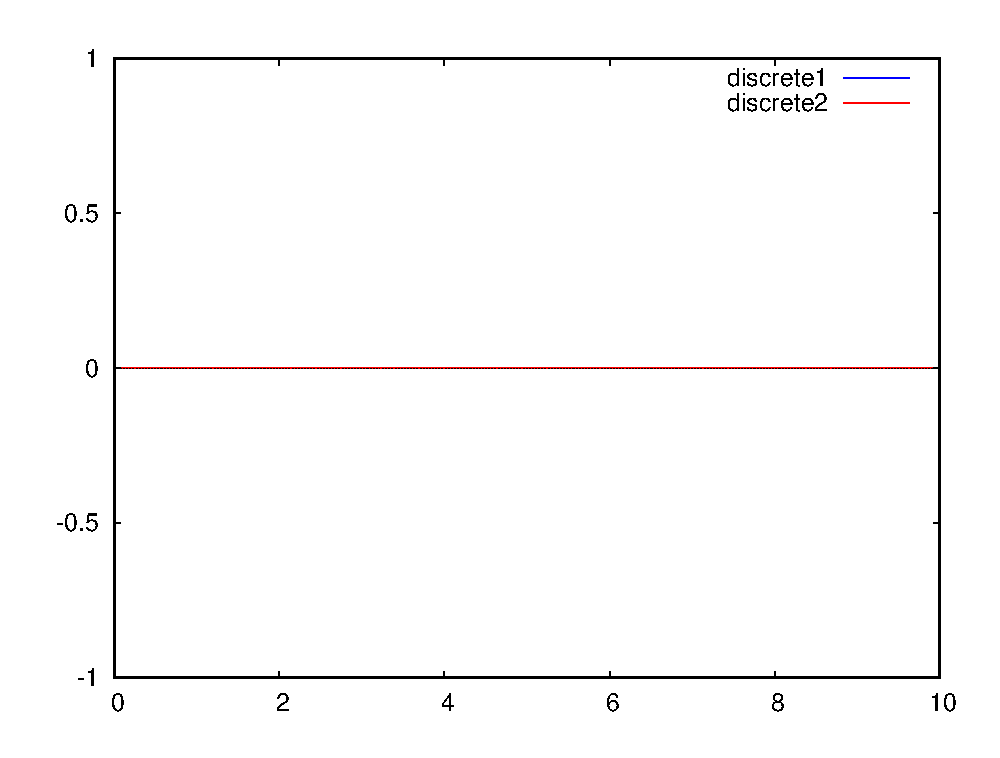
\includegraphics[width=\linewidth, height=30mm]{_old_sol__0_0_1__0__10__1e2_nu12} \\
            $\nu_1(t), \nu_2(t)$
        \column{0.33\textwidth}
            \centering
            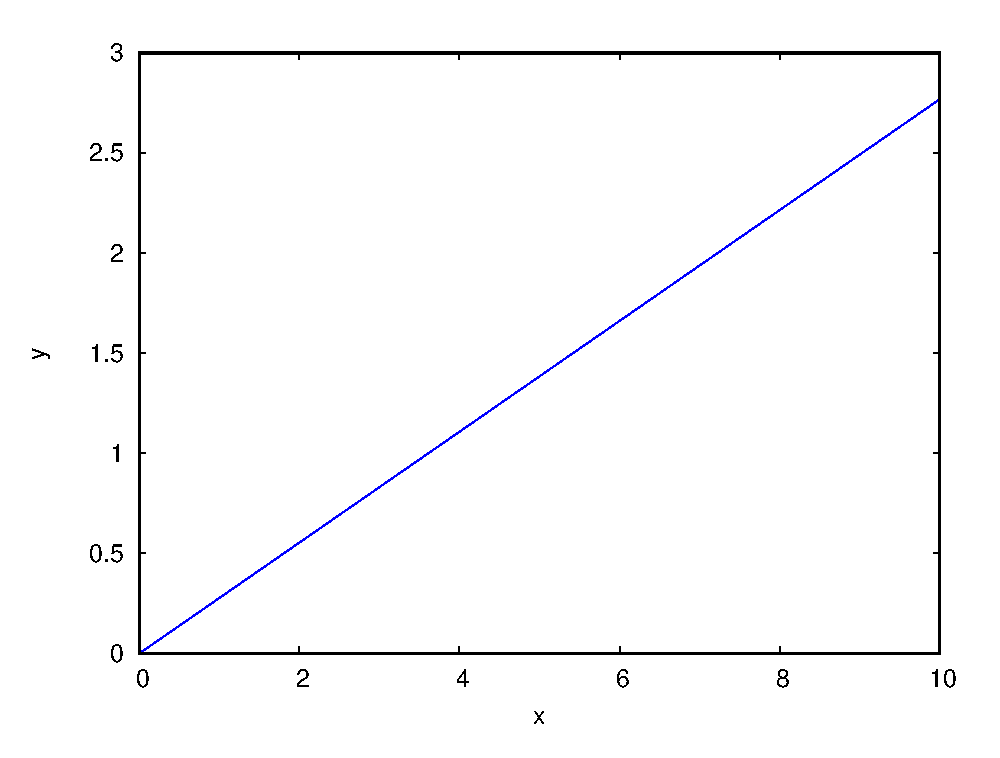
\includegraphics[width=\linewidth, height=30mm]{_old_sol__0_0_1__0__10__1e2_theta} \\
            $\theta(t)$ \\
            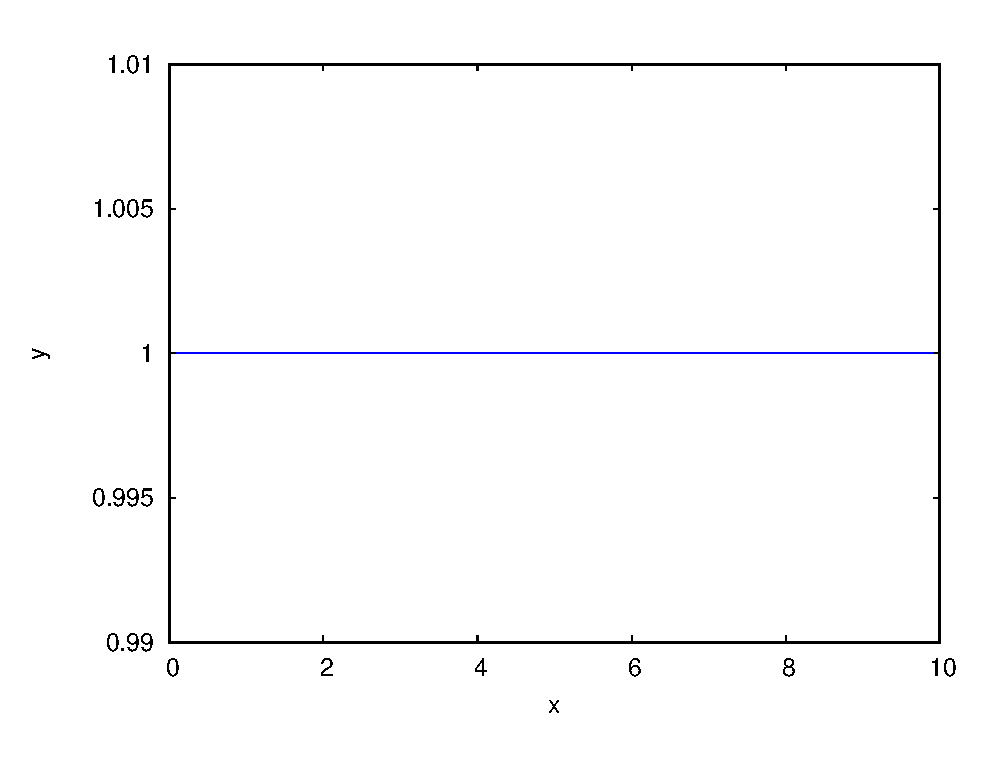
\includegraphics[width=\linewidth, height=30mm]{_old_sol__0_0_1__0__10__1e2_nu3} \\
            $\nu_3(t)$
        \column{0.33\textwidth}
            \centering
            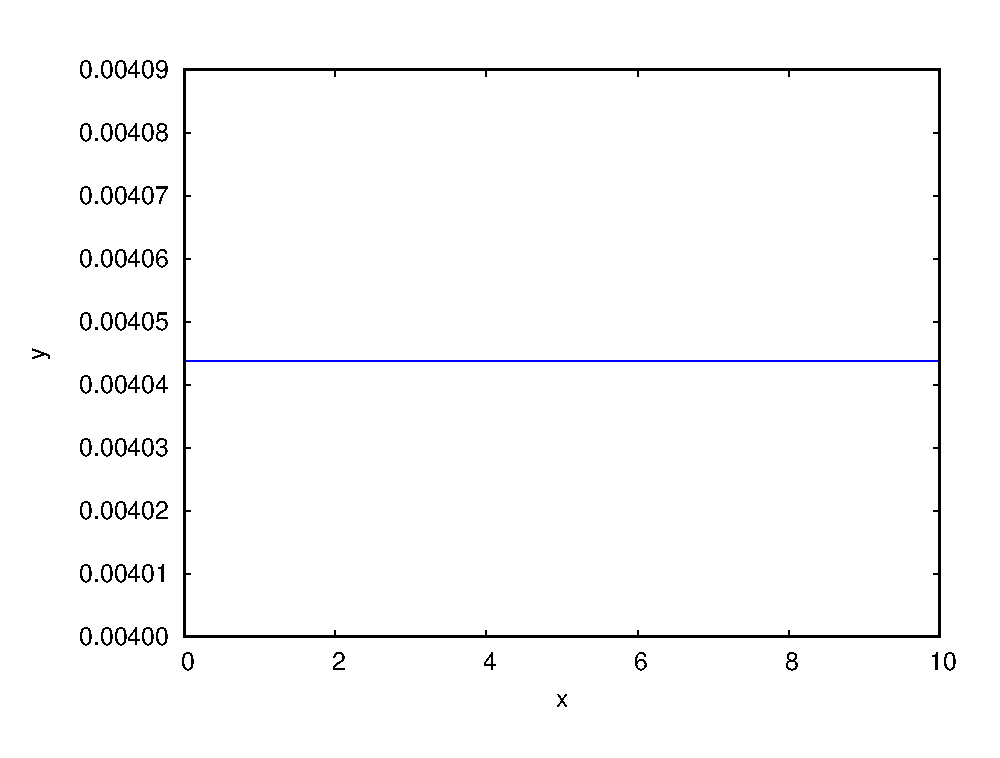
\includegraphics[width=\linewidth, height=30mm]{_old_sol__0_0_1__0__10__1e2_kin_en} \\
            Кинетическая энергия \\
            \vspace{15pt}
            Центр экипажа неподвижен, скорость вращения и энергия постоянны.
    \end{columns}
\end{frame}

\begin{frame}{Вращение вокруг своей оси ($\nu_{1,2}(0) = 0, \nu_3 = 1$)}{Экипаж с роликами}
    \begin{columns}
        \column{0.33\textwidth}
            \centering
            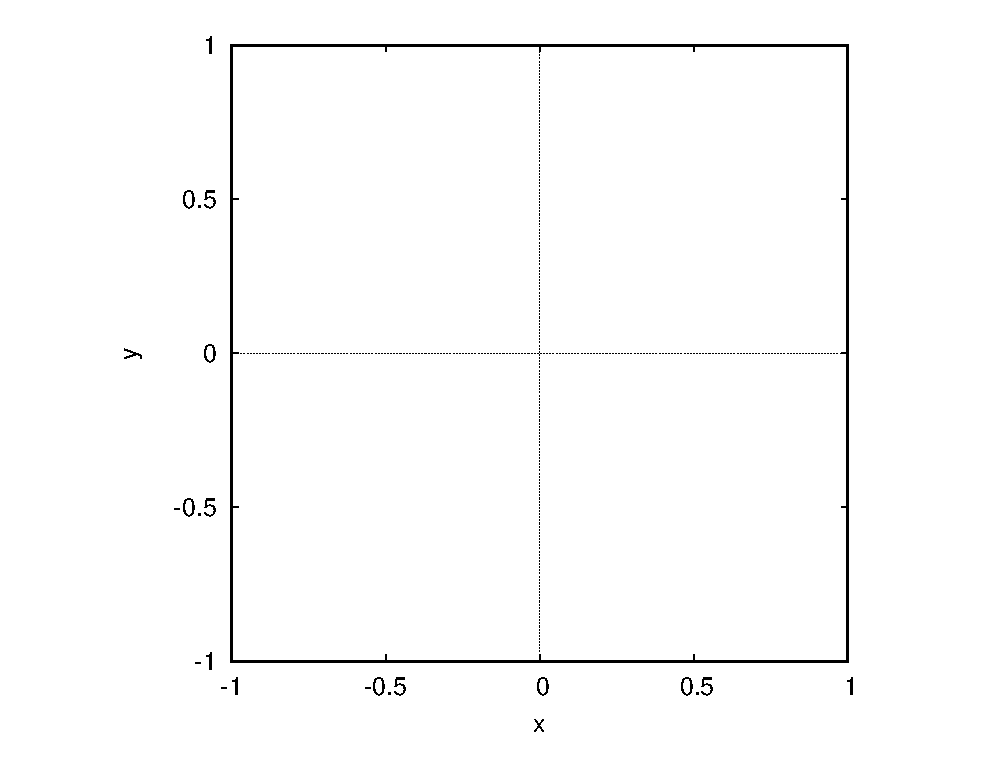
\includegraphics[width=\linewidth, height=30mm]{_sol__0_0_1__0__10__1e2_trajectory} \\
            Траектория $X, Y$ \\
            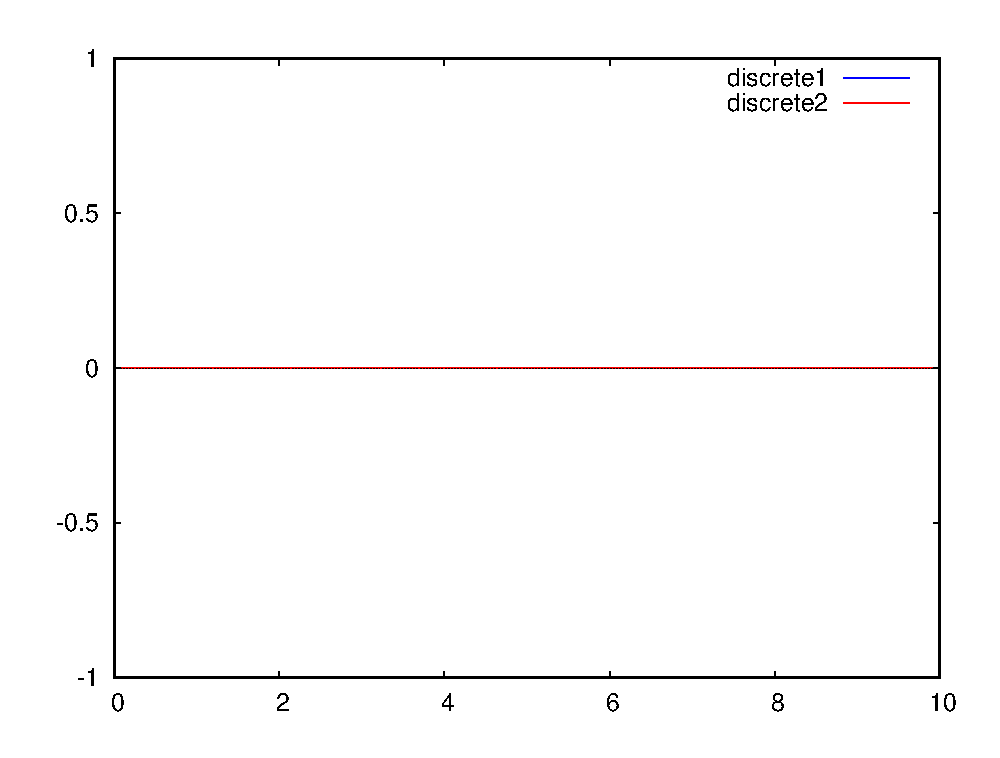
\includegraphics[width=\linewidth, height=30mm]{_sol__0_0_1__0__10__1e2_nu12} \\
            $\nu_1(t), \nu_2(t)$
        \column{0.33\textwidth}
            \centering
            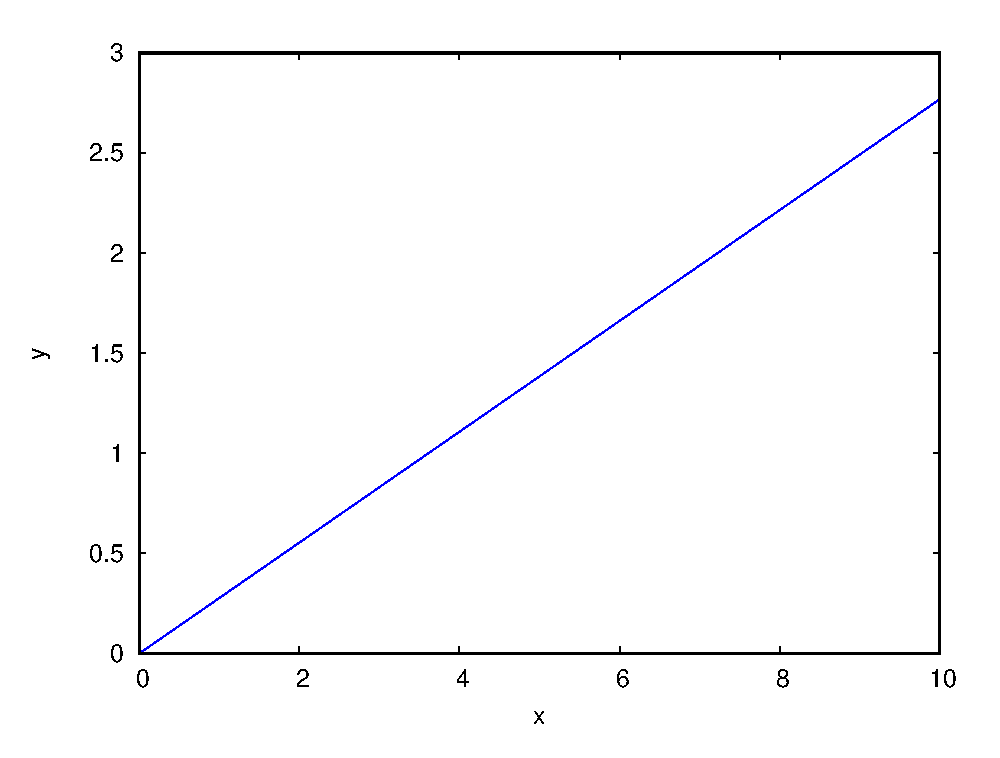
\includegraphics[width=\linewidth, height=30mm]{_sol__0_0_1__0__10__1e2_theta} \\
            $\theta(t)$ \\
            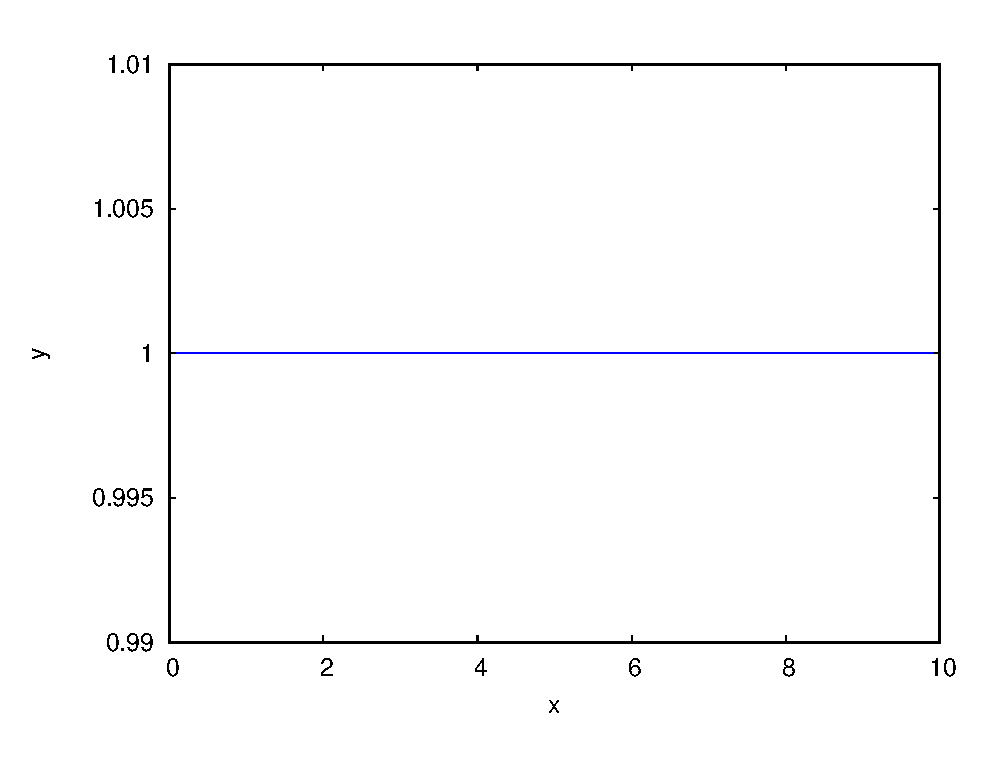
\includegraphics[width=\linewidth, height=30mm]{_sol__0_0_1__0__10__1e2_nu3} \\
            $\nu_3(t)$
        \column{0.33\textwidth}
            \centering
            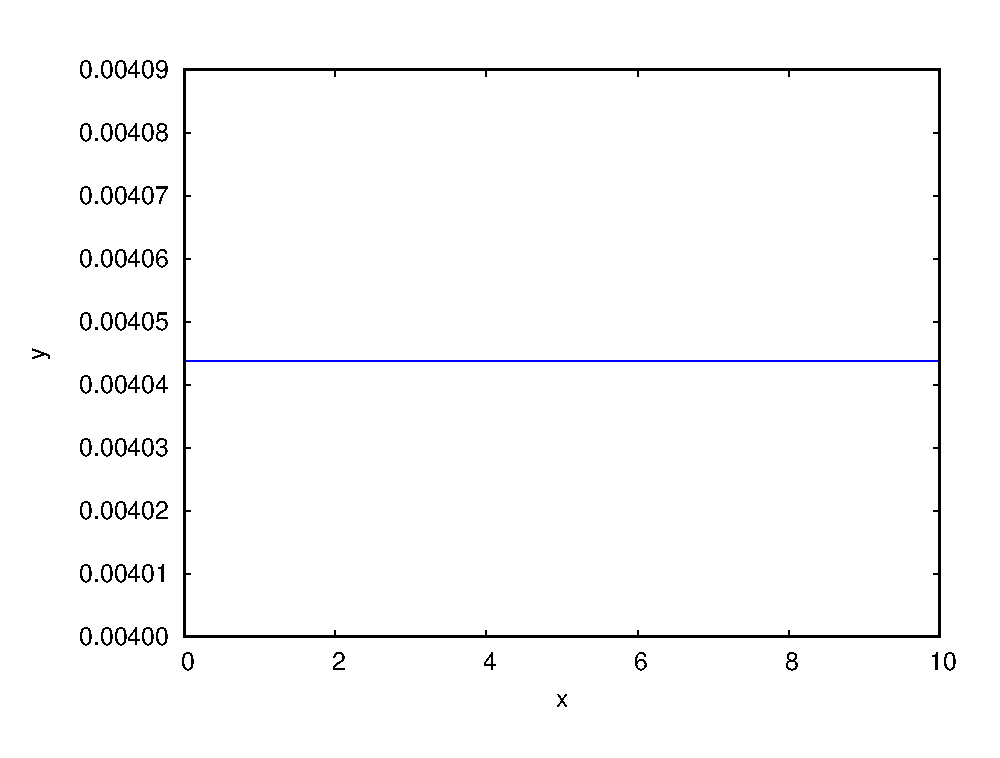
\includegraphics[width=\linewidth, height=30mm]{_sol__0_0_1__0__10__1e2_kin_en} \\
            Кинетическая энергия \\
            \vspace{15pt}
            Идентично случаю с роликами.
    \end{columns}
\end{frame}

\begin{frame}{Движение по прямой ($\nu_1(0) = 1, \nu_{2,3} = 0$)}{Экипаж без роликов}
    \begin{columns}
        \column{0.33\textwidth}
            \centering
            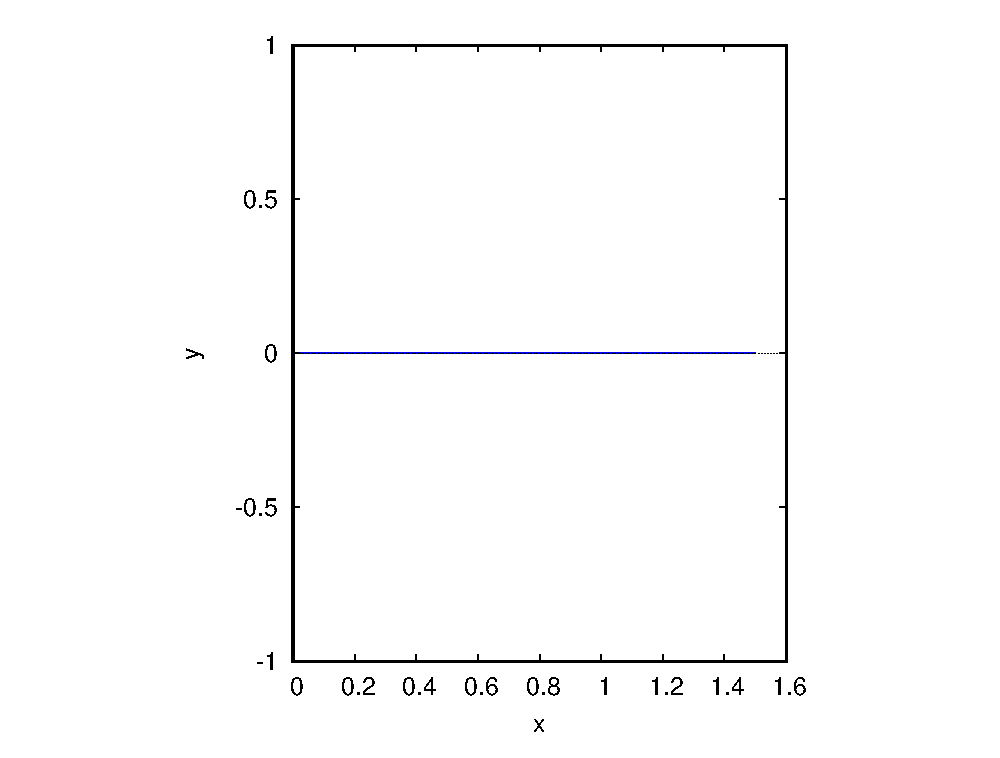
\includegraphics[width=\linewidth, height=30mm]{_old_sol__1_0_0__0__10__1e2_trajectory} \\
            Траектория $X, Y$ \\
            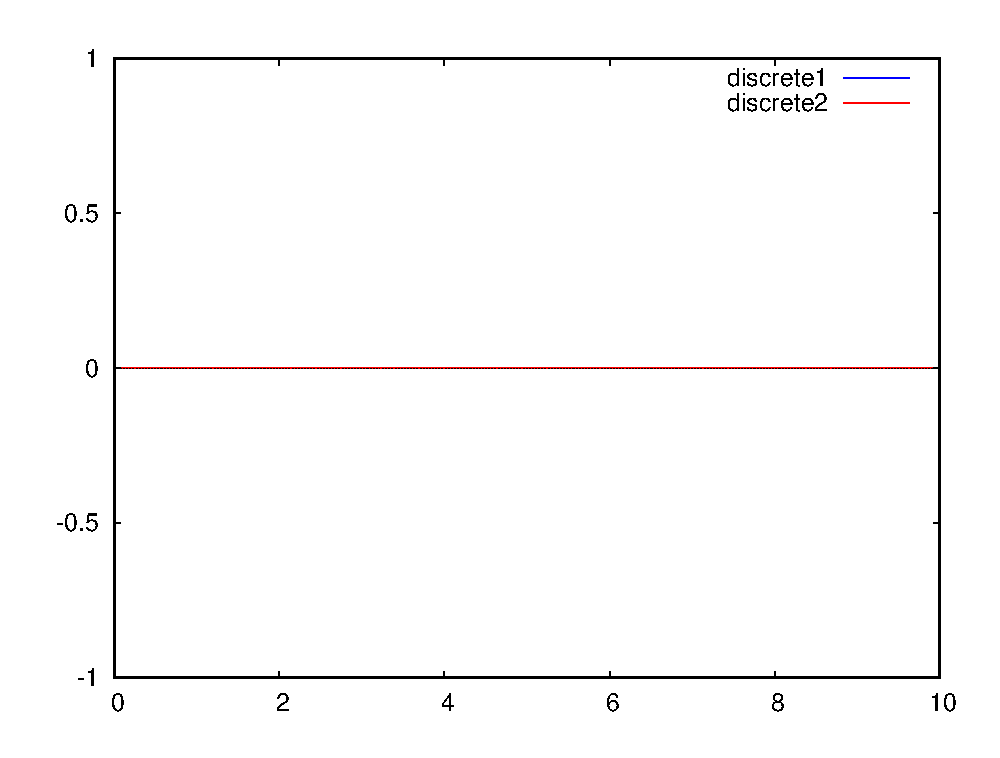
\includegraphics[width=\linewidth, height=30mm]{_old_sol__1_0_0__0__10__1e2_nu12_centered} \\
            $\nu_{1,2}(t) - \nu_{1,2}(0)$
        \column{0.33\textwidth}
            \centering
            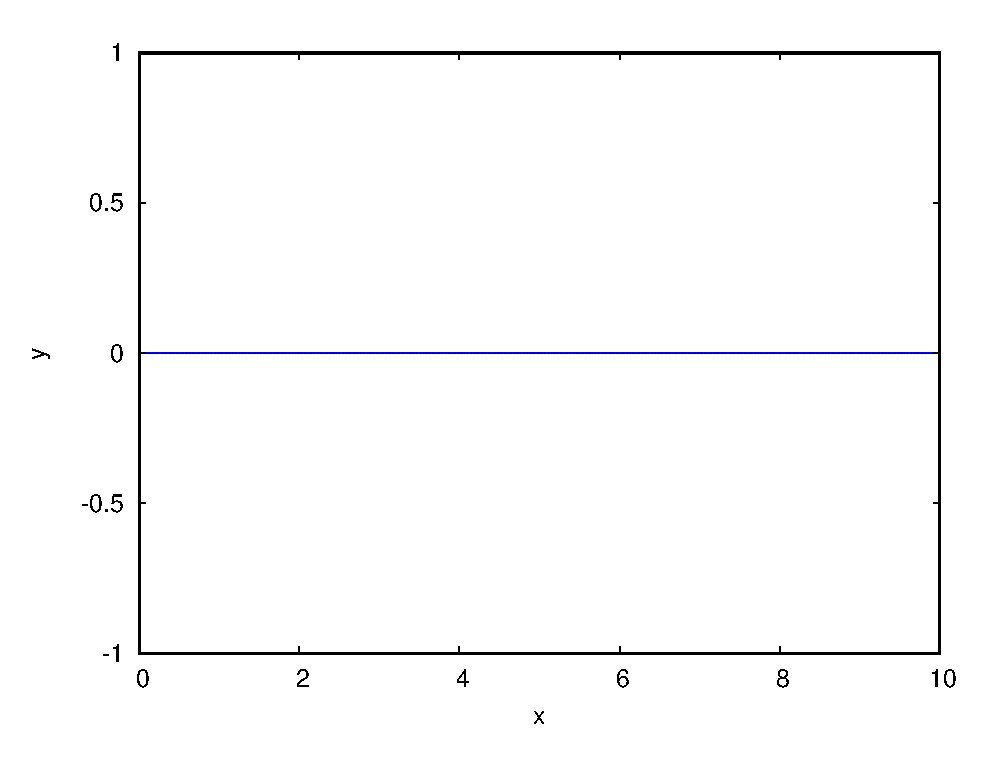
\includegraphics[width=\linewidth, height=30mm]{_old_sol__1_0_0__0__10__1e2_theta} \\
            $\theta(t)$ \\
            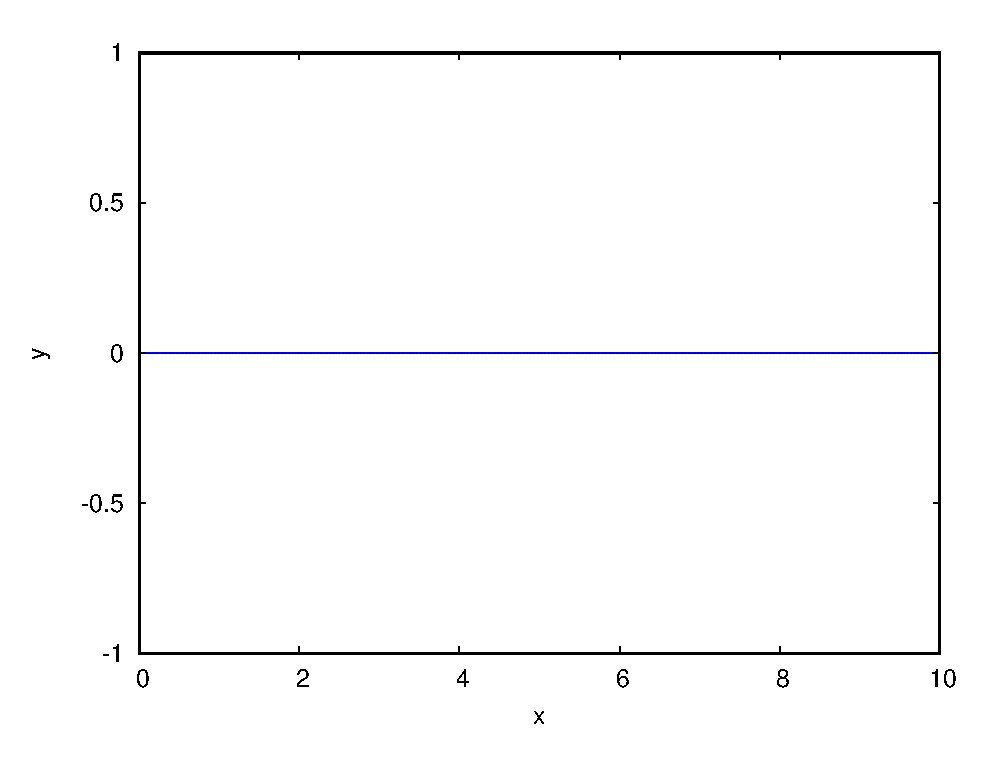
\includegraphics[width=\linewidth, height=30mm]{_old_sol__1_0_0__0__10__1e2_nu3} \\
            $\nu_3(t)$
        \column{0.33\textwidth}
            \centering
            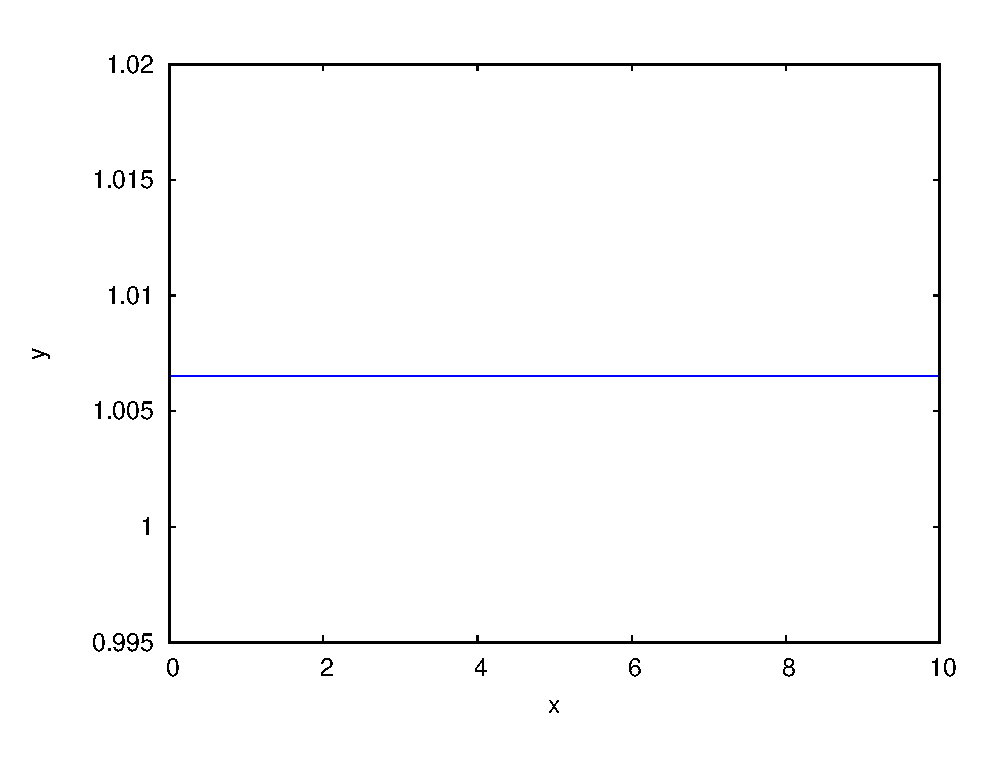
\includegraphics[width=\linewidth, height=30mm]{_old_sol__1_0_0__0__10__1e2_kin_en} \\
            Кинетическая энергия \\
            \vspace{15pt}
            Экипаж равномерно движется по прямой, не вращаясь, энергия постоянна.
    \end{columns}
\end{frame}

\begin{frame}{Движение по прямой ($\nu_1(0) = 1, \nu_{2,3} = 0$)}{Экипаж с роликами}
    \begin{columns}
        \column{0.33\textwidth}
            \centering
            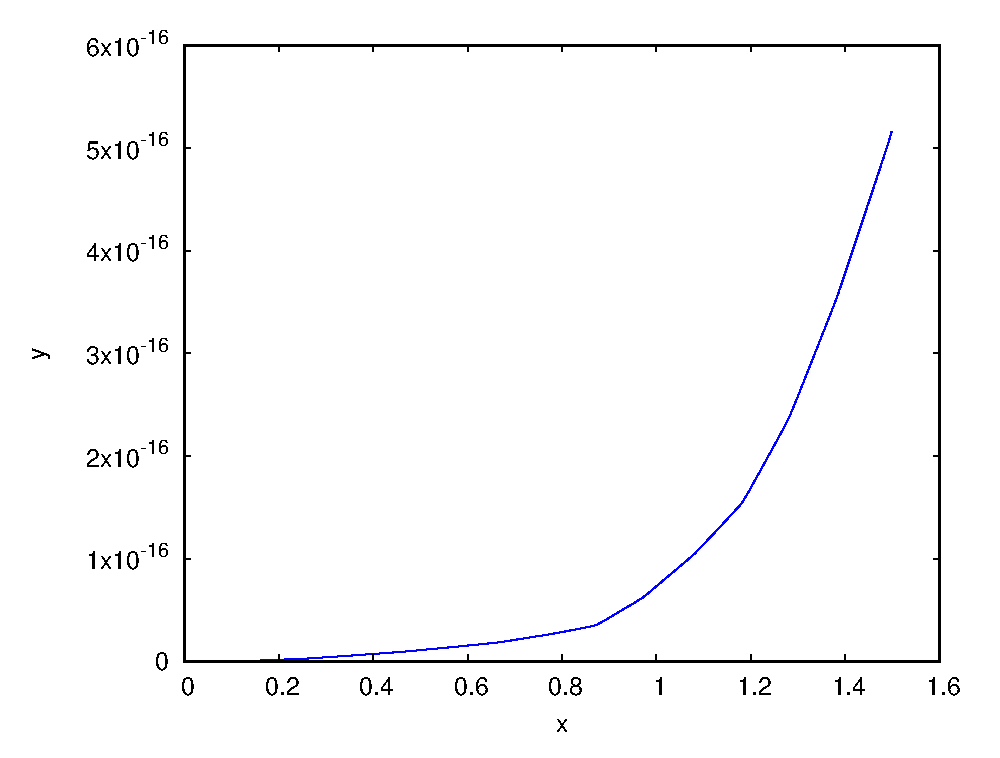
\includegraphics[width=\linewidth, height=30mm]{_sol__1_0_0__0__10__1e2_trajectory} \\
            Траектория $X, Y$ \\
            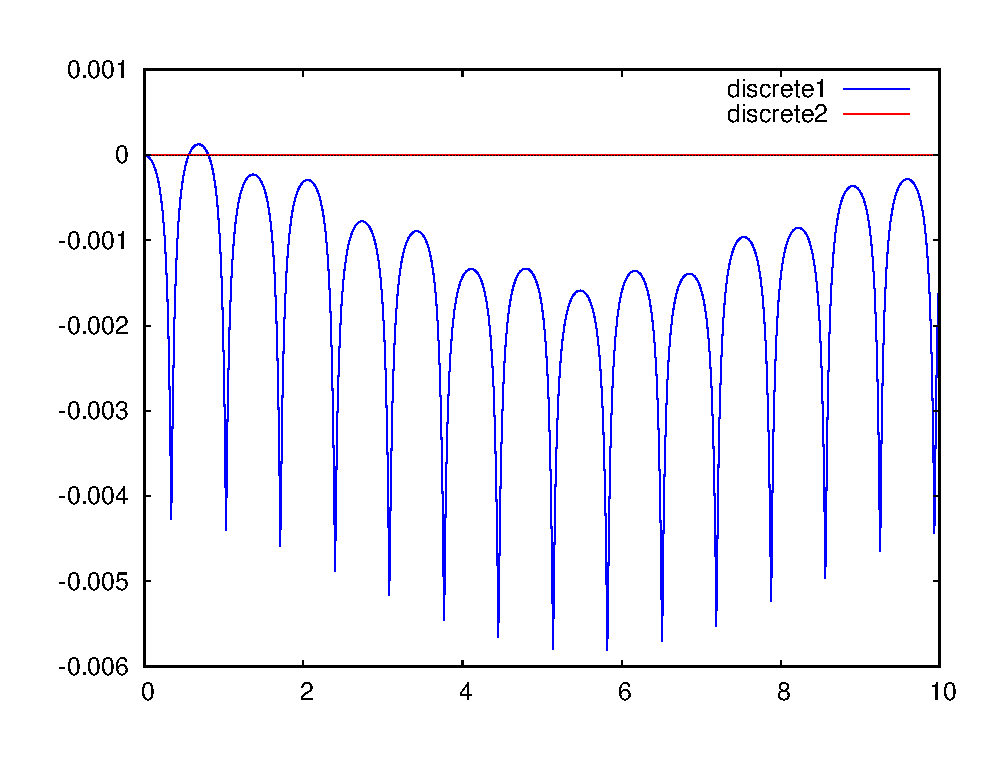
\includegraphics[width=\linewidth, height=30mm]{_sol__1_0_0__0__10__1e2_nu12_centered} \\
            $\nu_{1,2}(t) - \nu_{1,2}(0)$
        \column{0.33\textwidth}
            \centering
            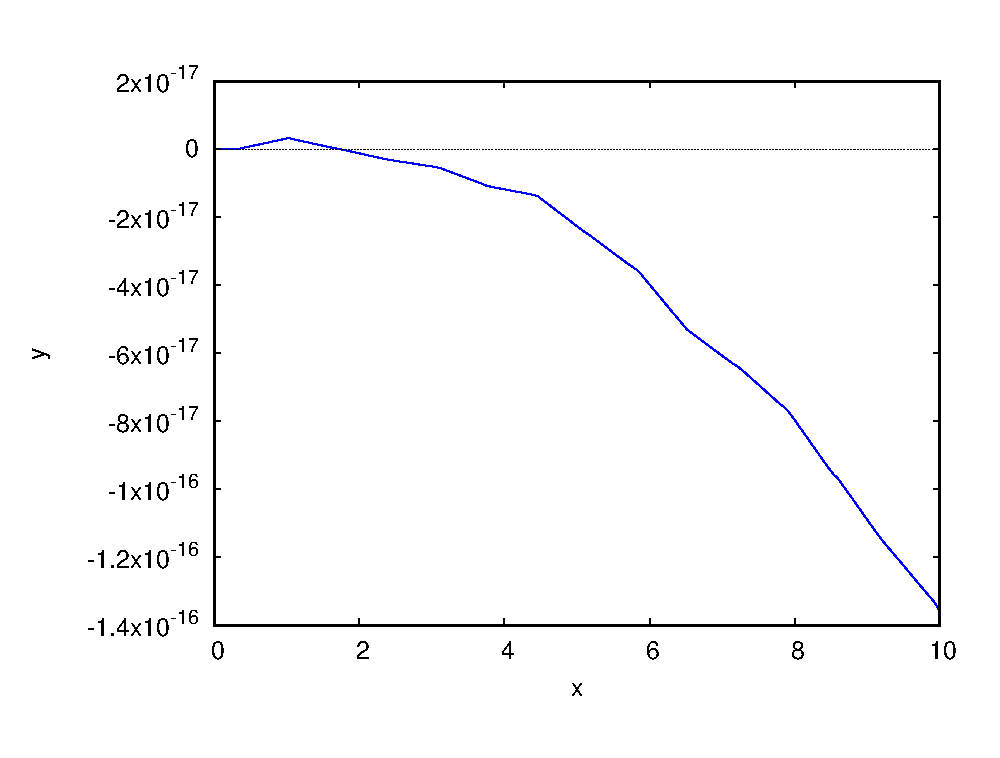
\includegraphics[width=\linewidth, height=30mm]{_sol__1_0_0__0__10__1e2_theta} \\
            $\theta(t)$ \\
            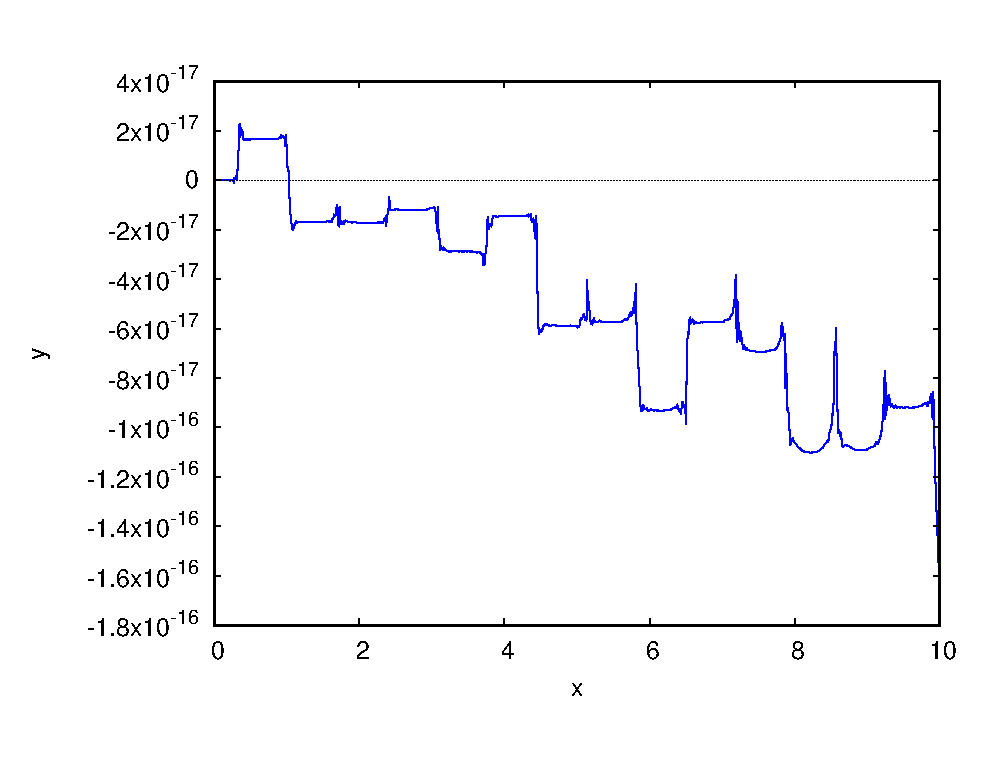
\includegraphics[width=\linewidth, height=30mm]{_sol__1_0_0__0__10__1e2_nu3} \\
            $\nu_3(t)$
        \column{0.33\textwidth}
            \centering
            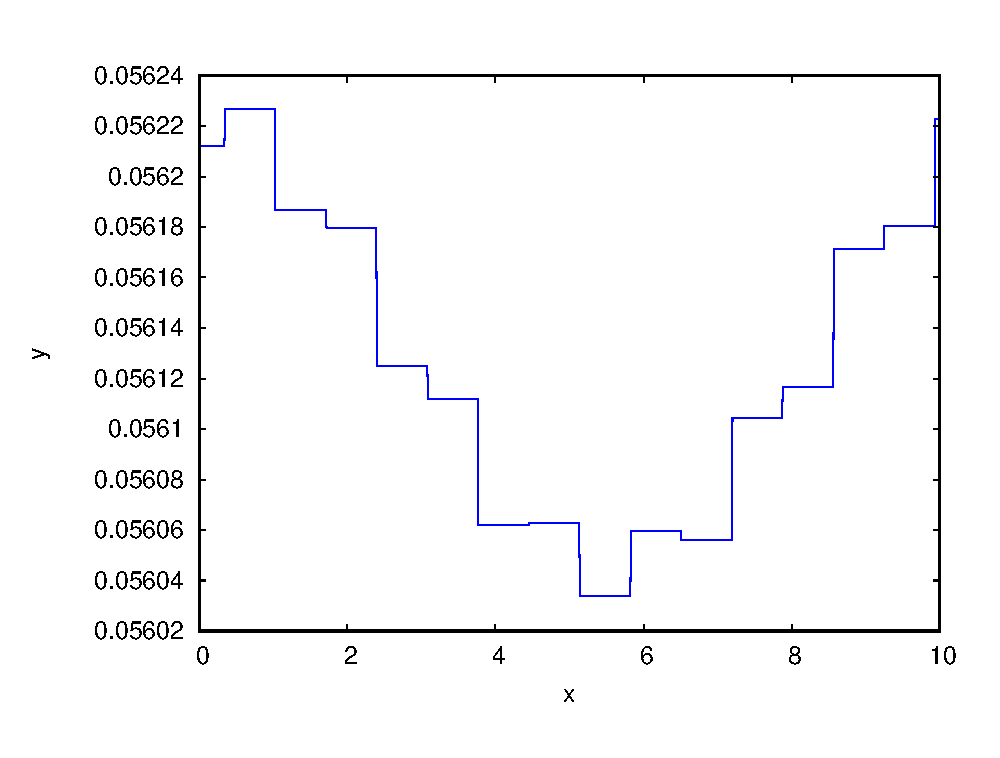
\includegraphics[width=\linewidth, height=30mm]{_sol__1_0_0__0__10__1e2_kin_en} \\
            Кинетическая энергия \\
            \vspace{15pt}
            Энергия и псевдоскорость $\nu_1$ не постоянны. Присутствует шум по координатам.
    \end{columns}
\end{frame}

\begin{frame}{Движение с закруткой ($\nu_1(0) = 1, \nu_2(0) = 0, \nu_3(0) = 1$)}{Экипаж без роликов}
    \begin{columns}
        \column{0.33\textwidth}
            \centering
            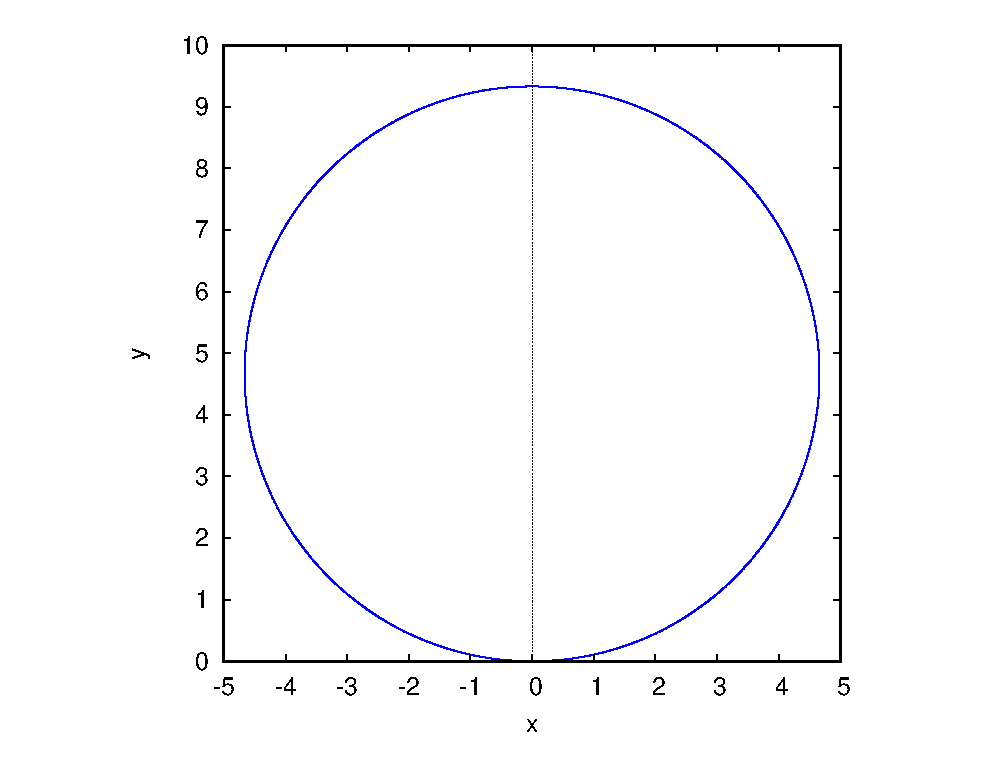
\includegraphics[width=\linewidth, height=30mm]{_old_sol__1_0_1__0__230__1e2_trajectory} \\
            Траектория $X, Y$ \\
            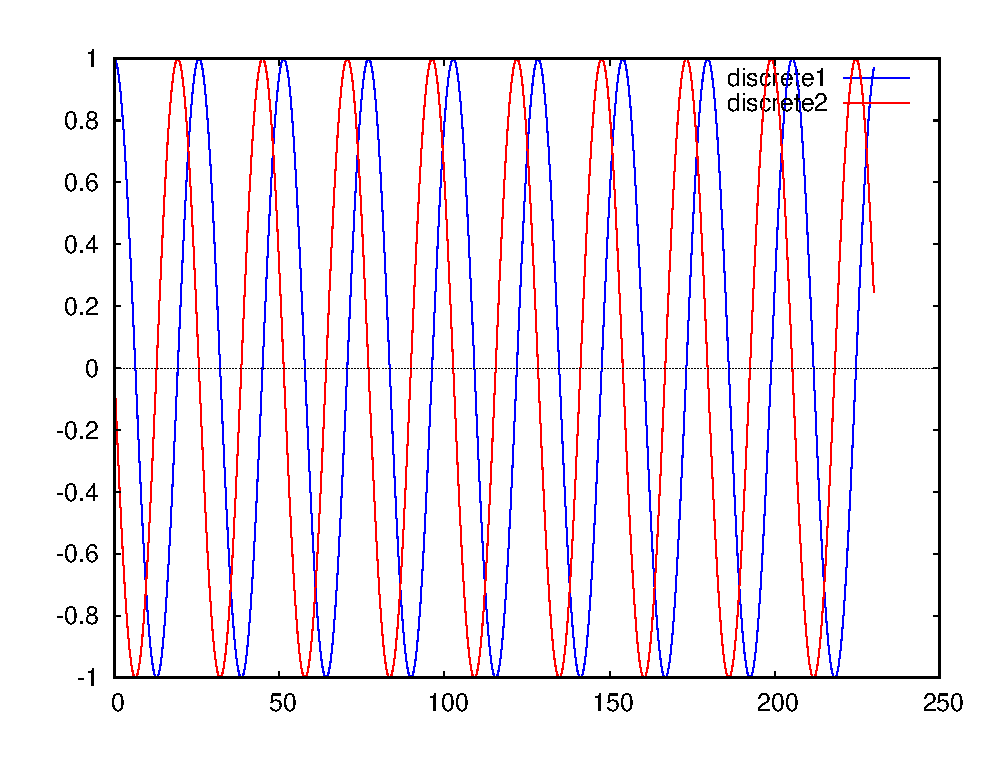
\includegraphics[width=\linewidth, height=30mm]{_old_sol__1_0_1__0__230__1e2_nu12} \\
            $\nu_{1,2}(t) - \nu_{1,2}(0)$
        \column{0.33\textwidth}
            \centering
            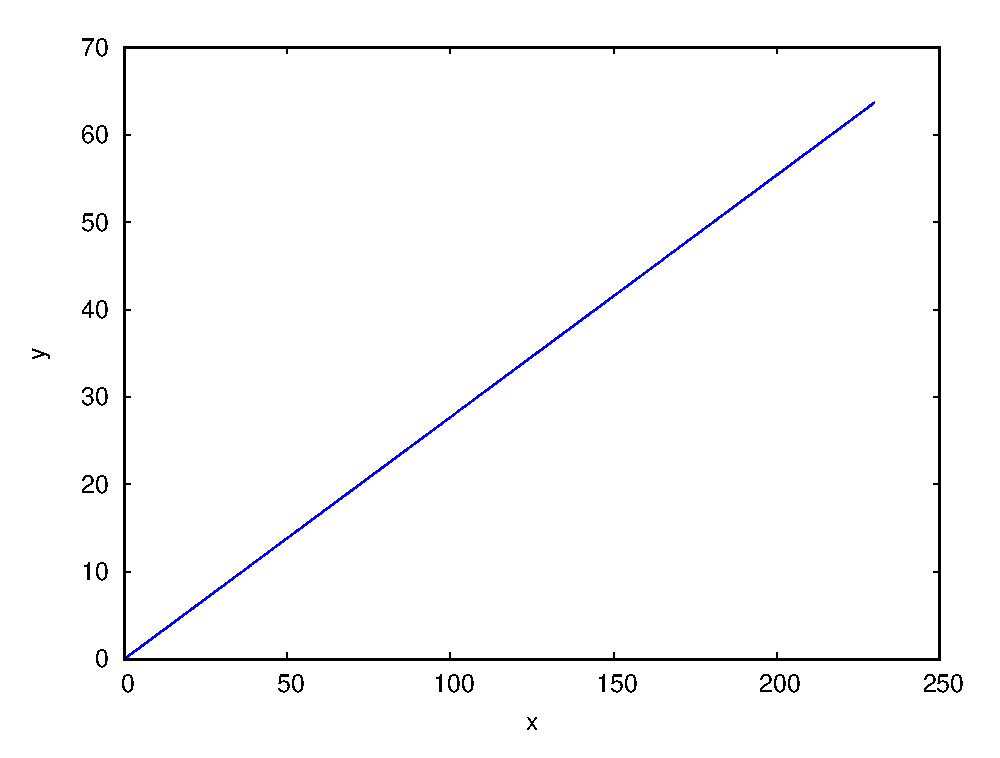
\includegraphics[width=\linewidth, height=30mm]{_old_sol__1_0_1__0__230__1e2_theta} \\
            $\theta(t)$ \\
            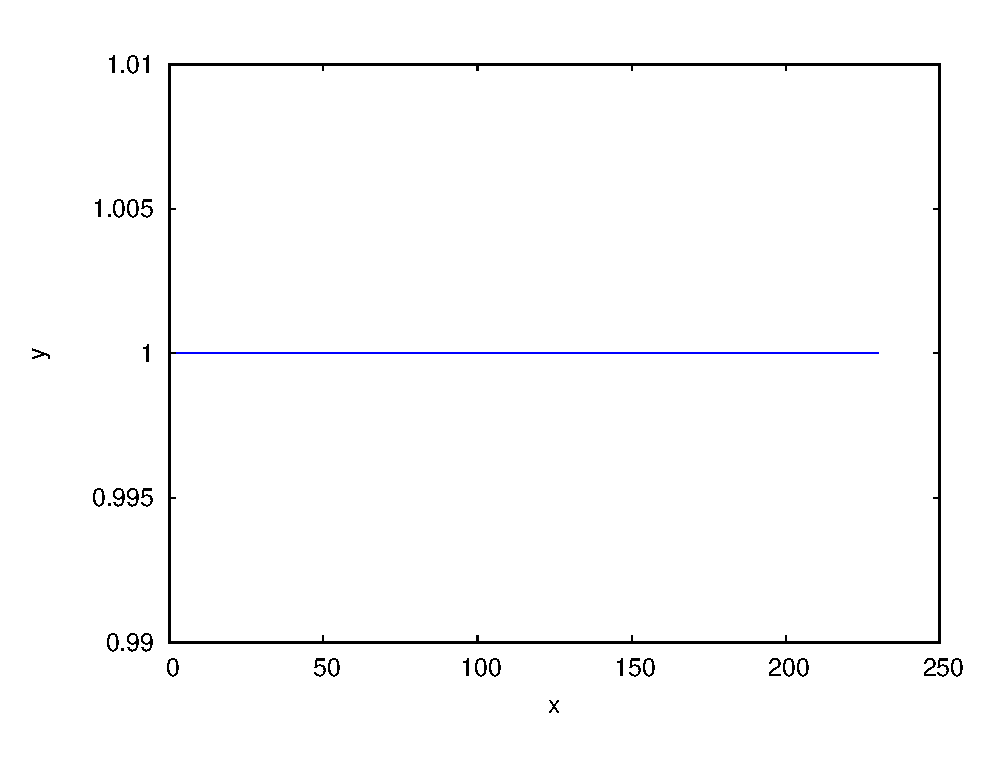
\includegraphics[width=\linewidth, height=30mm]{_old_sol__1_0_1__0__230__1e2_nu3} \\
            $\nu_3(t)$
        \column{0.33\textwidth}
            \centering
            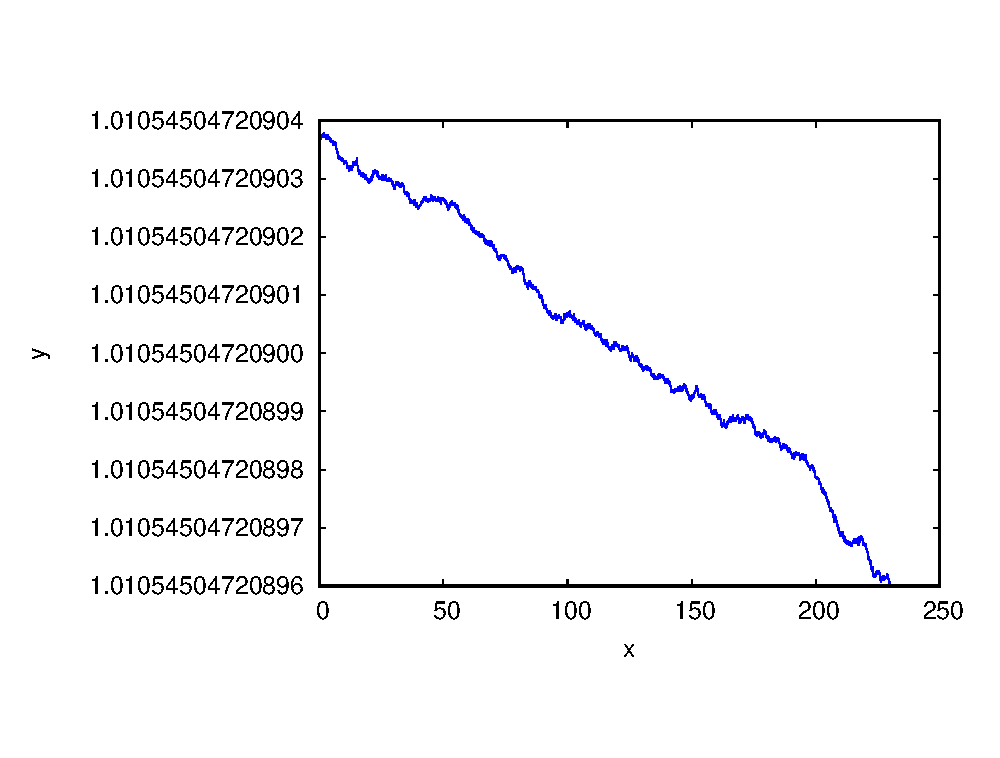
\includegraphics[width=\linewidth, height=30mm]{_old_sol__1_0_1__0__230__1e2_kin_en} \\
            Кинетическая энергия \\
            \vspace{15pt}
            Экипаж движется по окружности, равномерно вращаясь вокруг своей оси.
    \end{columns}
\end{frame}

\begin{frame}{Движение с закруткой ($\nu_1(0) = 1, \nu_2(0) = 0, \nu_3(0) = 1$)}{Экипаж c роликами}
    \begin{columns}
        \column{0.33\textwidth}
            \centering
            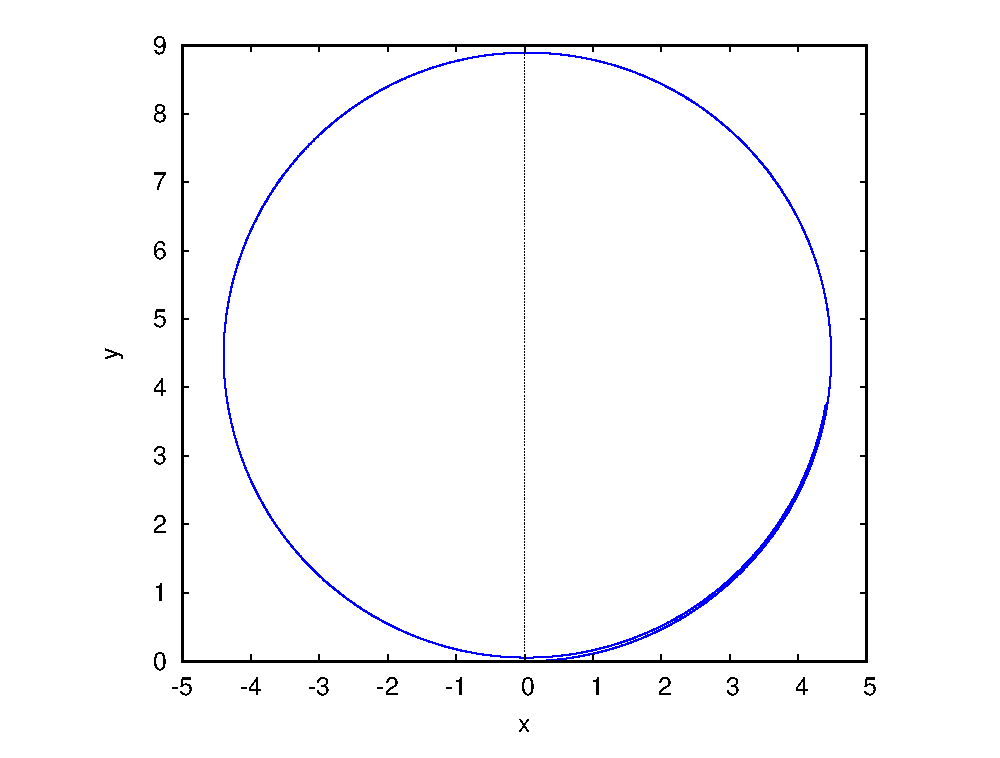
\includegraphics[width=\linewidth, height=30mm]{_sol__1_0_1__0__230__1e2_trajectory} \\
            Траектория $X, Y$ \\
            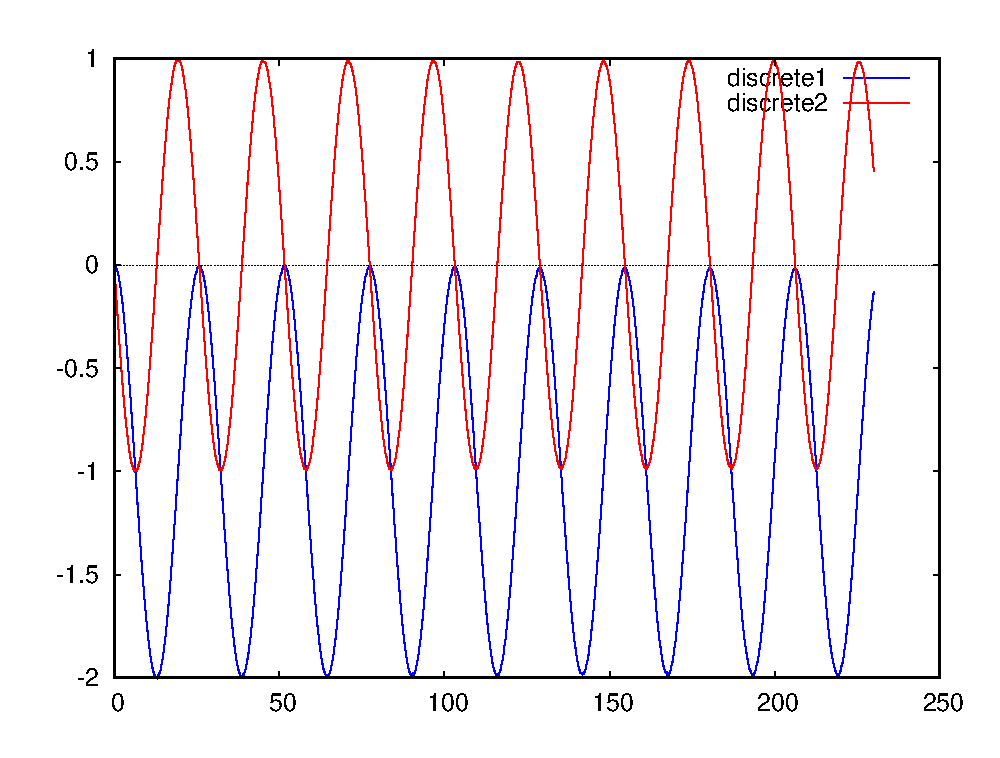
\includegraphics[width=\linewidth, height=30mm]{_sol__1_0_1__0__230__1e2_nu12_centered} \\
            $\nu_{1,2}(t) - \nu_{1,2}(0)$
        \column{0.33\textwidth}
            \centering
            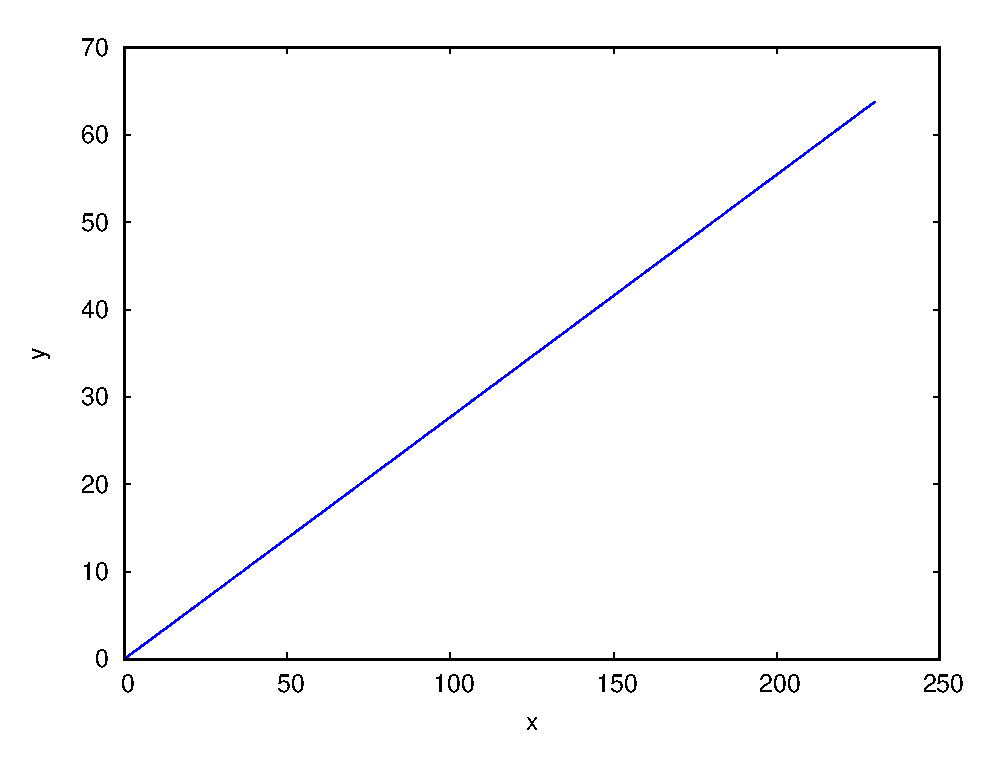
\includegraphics[width=\linewidth, height=30mm]{_sol__1_0_1__0__230__1e2_theta} \\
            $\theta(t)$ \\
            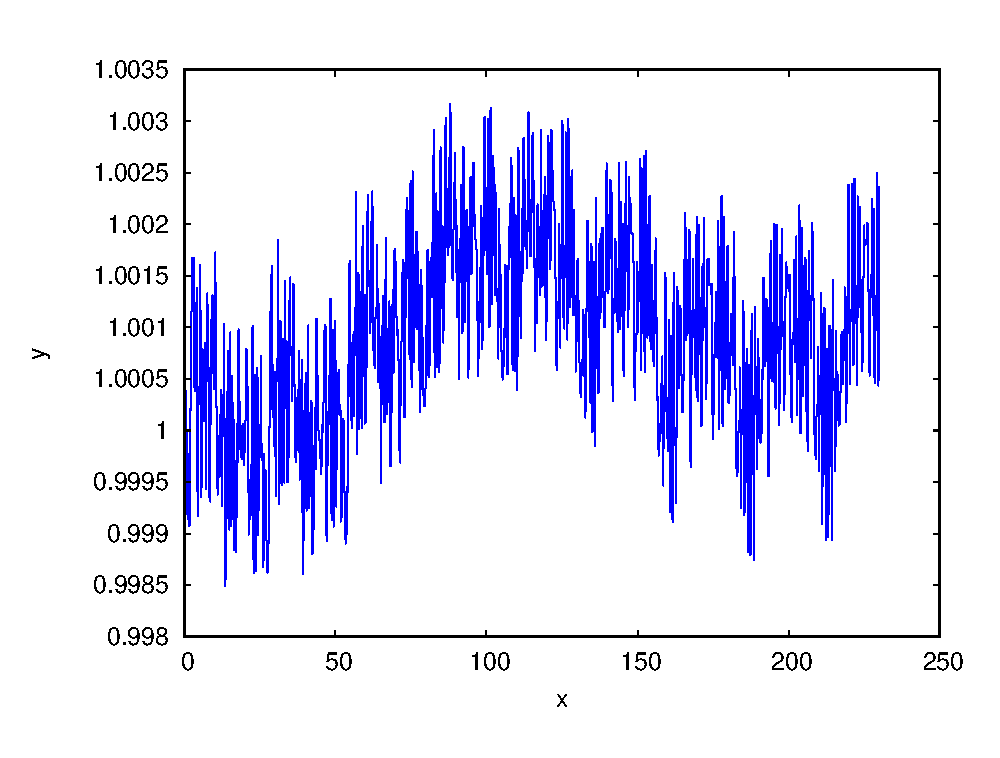
\includegraphics[width=\linewidth, height=30mm]{_sol__1_0_1__0__230__1e2_nu3} \\
            $\nu_3(t)$
        \column{0.33\textwidth}
            \centering
            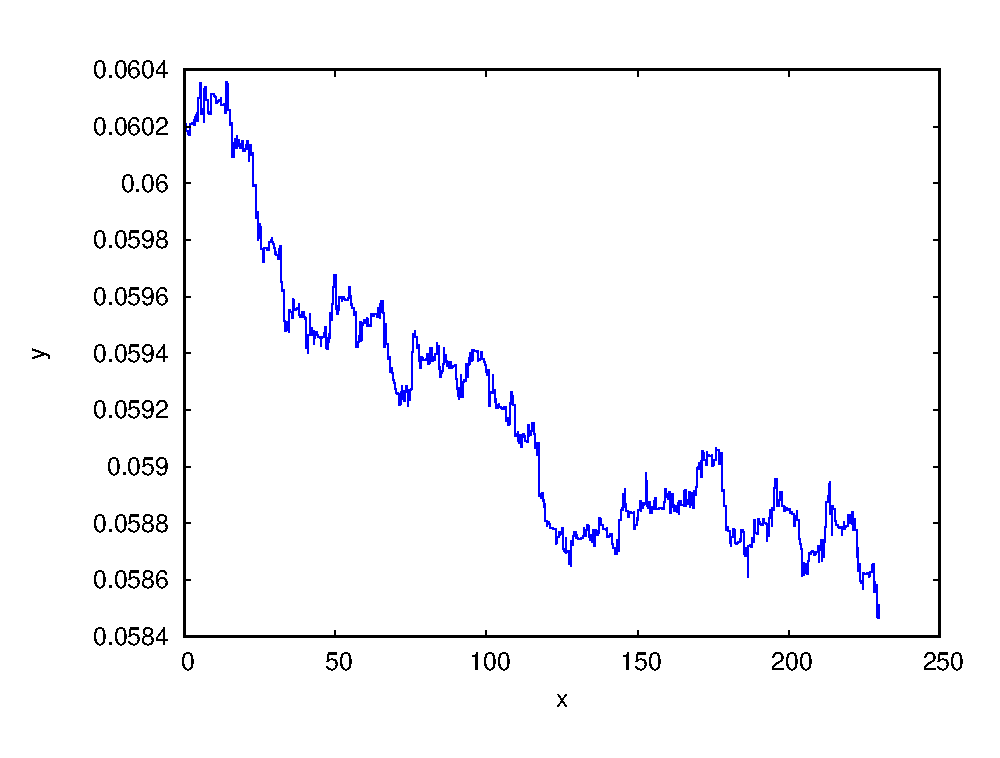
\includegraphics[width=\linewidth, height=30mm]{_sol__1_0_1__0__230__1e2_kin_en} \\
            Кинетическая энергия \\
            \vspace{15pt}
            Энергия не постоянна. Биения в псевдоскоростях.
    \end{columns}
\end{frame}

\begin{frame}{Движение с закруткой ($\nu_1(0) = 1, \nu_2(0) = 0, \nu_3(0) = 1$)}{Экипаж c роликами}
    \begin{columns}
        \column{0.33\textwidth}
            \centering
            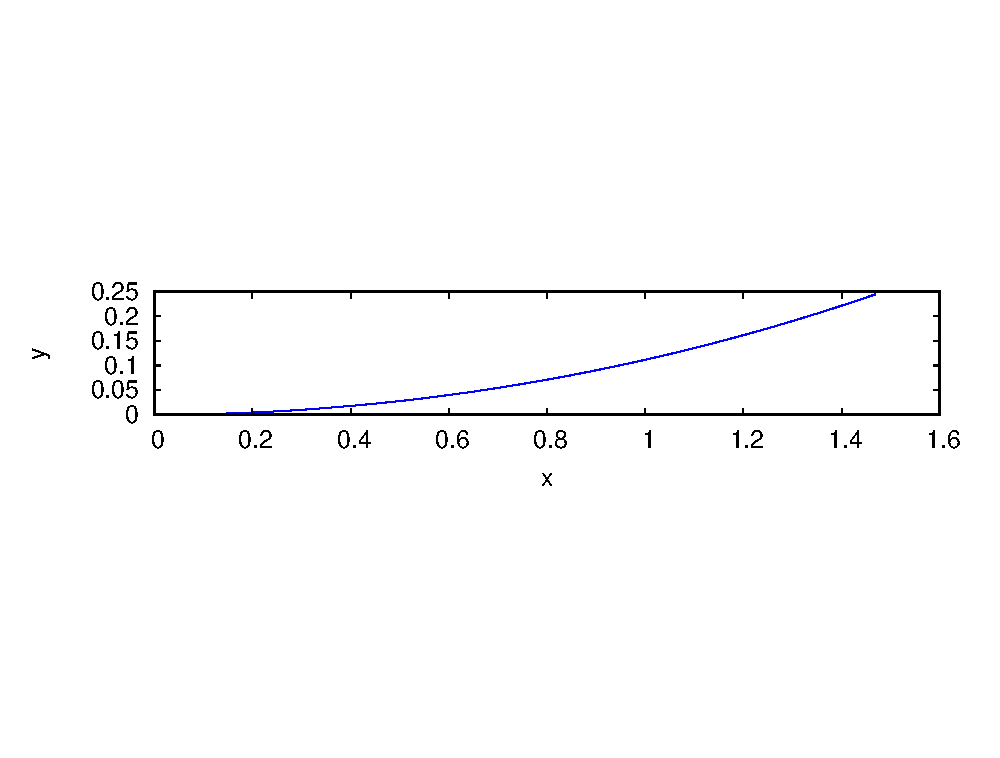
\includegraphics[width=\linewidth, height=30mm]{_sol__1_0_1__0__10__1e2_trajectory} \\
            Траектория $X, Y$ \\
            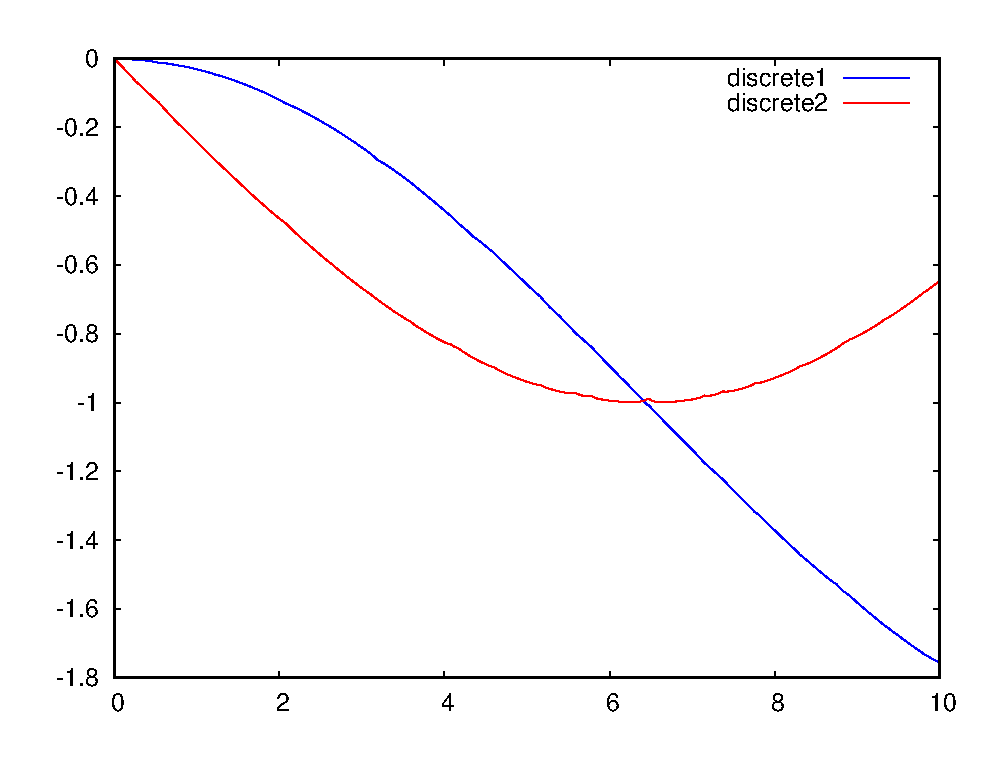
\includegraphics[width=\linewidth, height=30mm]{_sol__1_0_1__0__10__1e2_nu12_centered} \\
            $\nu_{1,2}(t) - \nu_{1,2}(0)$
        \column{0.33\textwidth}
            \centering
            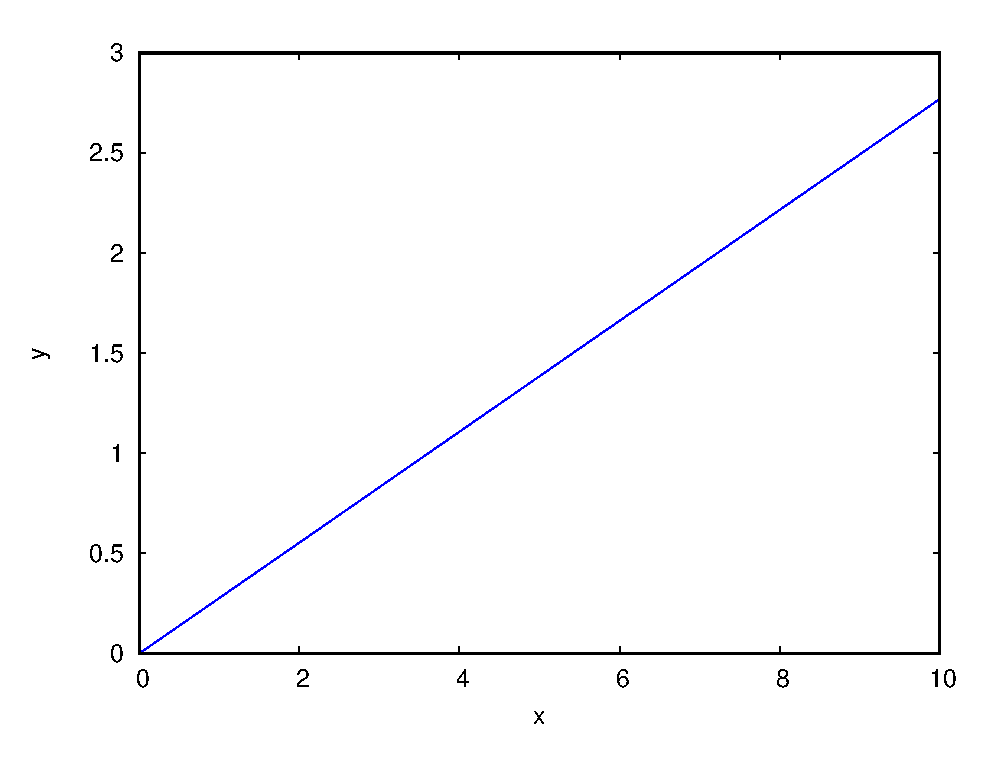
\includegraphics[width=\linewidth, height=30mm]{_sol__1_0_1__0__10__1e2_theta} \\
            $\theta(t)$ \\
            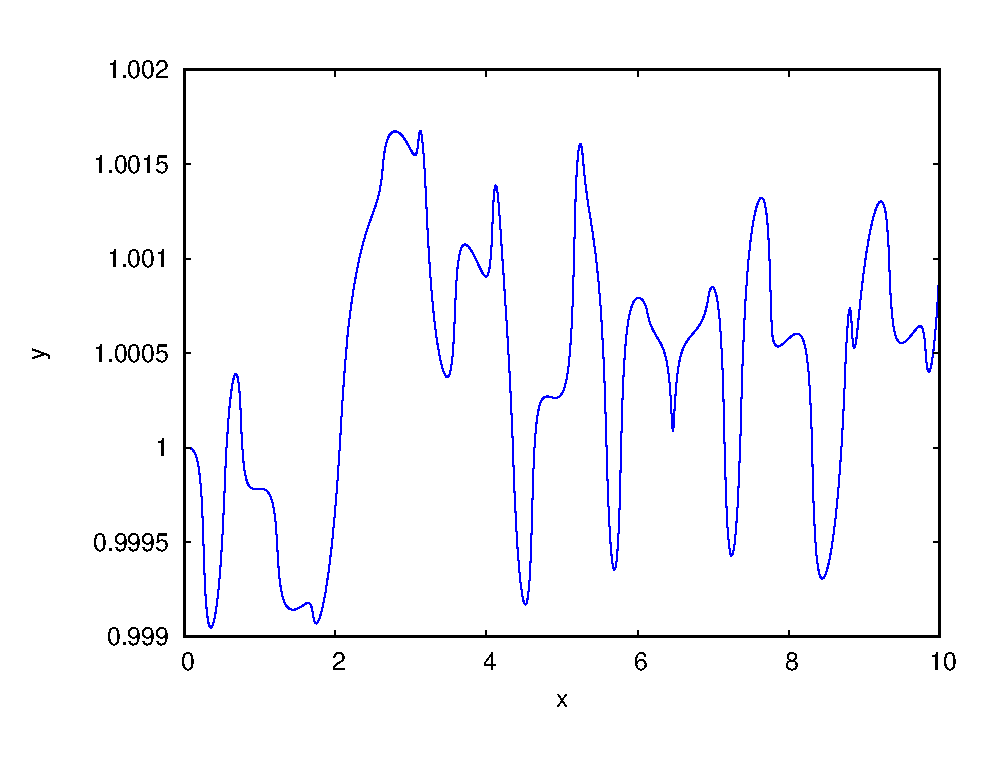
\includegraphics[width=\linewidth, height=30mm]{_sol__1_0_1__0__10__1e2_nu3} \\
            $\nu_3(t)$
        \column{0.33\textwidth}
            \centering
            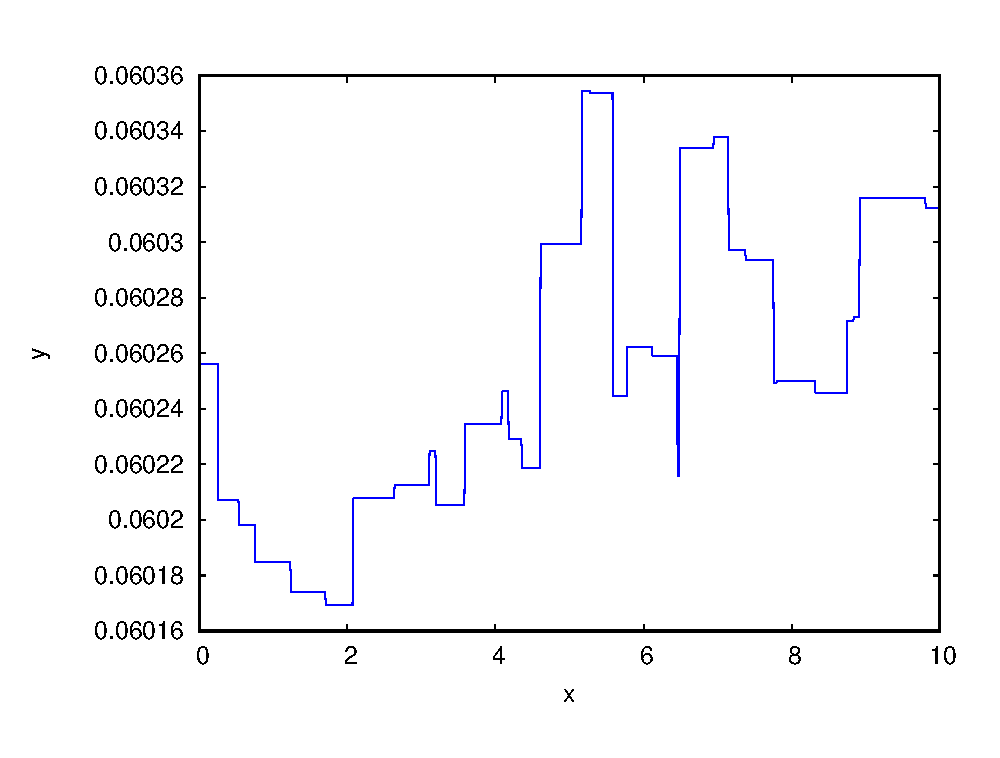
\includegraphics[width=\linewidth, height=30mm]{_sol__1_0_1__0__10__1e2_kin_en} \\
            Кинетическая энергия \\
            \vspace{15pt}
            Энергия не постоянна. Биения в псевдоскоростях.
    \end{columns}
\end{frame}

\begin{frame}{Результаты}
  \begin{itemize}
  \item
    Получены уравнения движения экипажа \alert{с полным набором роликов} в неголономной постановке.
  \item
    Показано, что разница с уравнениями для системы без роликов пропорциональна моменту инерции ролика.
  \item Предложена модель перехода с ролика на ролик.
  \item
    Получены численные решения при неподвижных свободных роликах для симметричной конфигурации.
  \end{itemize}
  \vspace{10pt}
  \centering
  \textcolor{Periwinkle}{Спасибо за внимание!}
\end{frame}

\end{document}


